%%
%% FRESCO v2: Cross-Cluster Workload Comparability
%% ROUGH DRAFT — generated from project data
%%
\documentclass[sigconf]{acmart}

\AtBeginDocument{%
  \providecommand\BibTeX{{%
    Bib\TeX}}}

%% Rights management — PLACEHOLDER: update for actual venue
\setcopyright{acmlicensed}
\copyrightyear{20XX}
\acmYear{20XX}
\acmDOI{XXXXXXX.XXXXXXX}

%% Conference info — PLACEHOLDER: update for actual target venue before submission.
%% If targeting MASCOTS 2026, switch to IEEEtran document class.
%% If targeting an ACM venue, update the fields below.
\acmConference[Conference 20XX]{Conference Name}{Date, Year}{City, Country}
\acmBooktitle{Proceedings of Conference Name, Date, Year, City, Country}
\acmISBN{978-X-XXXX-XXXX-X/20XX/XX}

\usepackage{booktabs}
\usepackage{multirow}
\usepackage{amsmath}

\begin{document}

\title{Beyond Unified Schemas: Why Zero-Shot Cross-Cluster Workload Transfer Fails and What It Takes to Make HPC Comparisons Defensible}

\author{Joshua McKerracher}
\email{jmckerra@purdue.edu}
\orcid{0009-0002-8856-9906}
\affiliation{%
  \institution{Purdue University}
  \city{West Lafayette}
  \state{Indiana}
  \country{USA}
}

\author{Saurabh Bagchi}
\orcid{0000-0002-4239-5632}
\affiliation{%
  \institution{Purdue University}
  \city{West Lafayette}
  \state{Indiana}
  \country{USA}
}
\email{sbagchi@purdue.edu}

\renewcommand{\shortauthors}{McKerracher and Bagchi}

%%% ============================================================
%%% ABSTRACT
%%% ============================================================
\begin{abstract}
Cross-cluster workload comparison is essential for capacity planning and system procurement, yet no published study has empirically validated whether predictive models trained on one HPC cluster can generalize to another.
We present FRESCO~v2, a provenance-rich dataset extending the original FRESCO schema from 19 to 65~columns across three production clusters spanning 75~months.
Using this dataset, we conduct an 84-experiment investigation proving that zero-shot cross-cluster memory prediction fails completely, yielding $R^2$~values as low as $-21$ due to fundamental domain shifts.
Even under best-case conditions---hardware regime matching, overlap-aware cohort selection, and unsupervised domain adaptation via CORAL and quantile mapping---transfer remains negative or unstable.
We further demonstrate that few-shot calibration with up to 500~labeled target examples and four distinct strategies (output recalibration, fine-tuning, stacking, and target-only baselines) fails to outperform the zero-shot reference, with the best few-shot result ($R^2 = 0.076$) still falling below zero-shot ($R^2 = 0.107$).
Because model transfer is unviable under any tested condition, we propose a Local Telemetry Blueprint that defines the minimal data inputs and training methodology required for HPC centers to build robust, site-specific predictive models. On 416,616 filtered, regime-matched Anvil jobs from the canonical FRESCO~v3 production dataset, this blueprint achieves $R^2 = 0.2520$ under a strict temporal split.
All 84 experiment configurations, code, and reproducibility artifacts are publicly available.
\end{abstract}

\begin{CCSXML}
<ccs2012>
   <concept>
       <concept_id>10010520.10010575</concept_id>
       <concept_desc>Computer systems organization~Dependable and fault-tolerant systems and networks</concept_desc>
       <concept_significance>500</concept_significance>
   </concept>
   <concept>
       <concept_id>10010147.10010257</concept_id>
       <concept_desc>Computing methodologies~Machine learning</concept_desc>
       <concept_significance>300</concept_significance>
   </concept>
</ccs2012>
\end{CCSXML}

\ccsdesc[500]{Computer systems organization~Dependable and fault-tolerant systems and networks}
\ccsdesc[300]{Computing methodologies~Machine learning}

\keywords{high-performance computing, cross-cluster transfer, domain shift, workload comparison, FRESCO dataset, measurement provenance, domain adaptation}

\maketitle

%%% ============================================================
%%% §1  INTRODUCTION
%%% ============================================================
\section{Introduction}

High-performance computing centers routinely make operational decisions---capacity planning, hardware procurement, scheduling policy adjustments---that would benefit from comparing workload behavior across clusters.
When a center considers upgrading from one system generation to the next, or when a funding agency evaluates proposals from different institutions, the ability to say \emph{``jobs of type~X consume Y\% more memory on Cluster~A than on Cluster~B''} would be enormously valuable.
Yet such comparisons are rarely attempted with empirical rigor, because the datasets, measurement semantics, and analytical frameworks required to support them have not existed.

The growing availability of public HPC workload datasets---including FRESCO~\cite{mckerracher2025fresco}, the Atlas cluster trace~\cite{atlas2020}, the CFDR failure dataset~\cite{cfdr2010}, and Google's Borg traces~\cite{google_borg_2015}---naturally raises the question of whether a predictive model trained on one cluster's historical data can simply be \emph{transferred} to another.
If so, a well-resourced center could train a memory or runtime prediction model once, and smaller centers could deploy it without collecting extensive local telemetry.
The appeal of such zero-shot transfer is obvious: it promises to democratize operational intelligence across the HPC ecosystem.

However, our baseline experiments demonstrate that this assumption is empirically false.
When a Ridge regression model trained on Anvil (a modern 1,000-node AMD EPYC cluster at Purdue) is naively evaluated on Conte (a 580-node Intel cluster from the same institution), cross-cluster memory prediction yields $R^2 = -9.31$ (95\% CI: $[-10.34, -8.53]$); the reverse direction produces $R^2 = -4.33$ (95\% CI: $[-4.63, -4.04]$).
These are not merely weak predictions---they are \emph{catastrophically} worse than simply predicting the target cluster's mean, indicating systematic miscalibration driven by fundamental differences in how memory is measured, what hardware exists, and what workloads run on each system.

This catastrophic failure is driven by three distinct phenomena that prior datasets, including the original FRESCO~v1 release, lacked the measurement provenance to diagnose.
First, \emph{covariate shift}~\cite{domain_adaptation_survey_2021}: the feature distributions across clusters are nearly non-overlapping (partition Kolmogorov-Smirnov distance~\cite{massey1951kolmogorov} $\text{KS} = 1.00$, node type $\text{KS} = 0.999$), meaning the source model has never seen inputs resembling the target domain (Figure~\ref{fig:domain-shifts}a).
Second, \emph{conditional shift} (Figure~\ref{fig:domain-shifts}b): even when we restrict analysis to hardware-matched regimes where features overlap, the mapping from job characteristics to memory consumption differs fundamentally---Anvil's cgroup-based memory accounting includes page cache while Conte's RSS-based measurement does not, creating a non-constant, application-dependent offset~\cite{peng2022memory}.
Third, \emph{era shift} (Figure~\ref{fig:domain-shifts}c): the clusters span different time periods (Conte: 2015--2017, Anvil: 2022--2023) with different user communities, software stacks, and workload compositions.

In this paper, we present three core contributions.
\textbf{(1)}~\textbf{FRESCO~v2}, a provenance-rich dataset extending the original 19-column schema to 65~columns with explicit hardware context, normalized memory fractions, and documented measurement semantics across 20.9~million jobs from three clusters.
\textbf{(2)}~\textbf{Empirical proof that transfer fails}: through 84~controlled experiments spanning zero-shot transfer, overlap-aware regime matching, unsupervised domain adaptation (CORAL, quantile mapping), and few-shot calibration with up to 500~labeled target examples, we demonstrate that no tested approach produces reliable cross-cluster memory prediction.
\textbf{(3)}~A \textbf{Local Telemetry Blueprint} that defines the minimal feature set, preprocessing, and training methodology required for HPC centers to build robust site-specific models, achieving $R^2 = 0.2520$ on 416,616 filtered, regime-matched Anvil jobs from the canonical FRESCO~v3 dataset under temporal hold-out splits.


%%% ============================================================
%%% §2  BACKGROUND & RELATED WORK
%%% ============================================================
\section{Background \& Related Work}

\subsection{HPC Workload Datasets}

The HPC community has produced several important public workload datasets, but none provides the combination of cross-institutional scope, per-job resource telemetry, and explicit measurement provenance required for rigorous transfer studies.
The Parallel Workloads Archive~\cite{feitelson2014experience} collects sanitized scheduler logs from dozens of systems spanning two decades, enabling foundational research on job scheduling, but records only submission metadata (arrival time, requested resources, runtime) without any performance telemetry such as memory consumption, CPU utilization, or I/O rates.
The Grid Workloads Archive~\cite{iosup2008grid} extends this to distributed grid environments but similarly lacks node-level resource measurements.
The Atlas cluster trace~\cite{atlas2020} provides scheduler logs from a mid-scale cluster and importantly documents workload diversity across system configurations, but does not include per-job memory or CPU telemetry.
The Computer Failure Data Repository (CFDR)~\cite{cfdr2010} focuses on hardware failure events rather than job-level resource usage.
Google's Borg traces~\cite{google_borg_2015} offer unprecedented scale and include resource usage data, but describe a proprietary cloud scheduling environment with container-based isolation that differs fundamentally from shared-node academic HPC.
TACC Stats~\cite{tacc_stats_2014} provides fine-grained per-node performance counters from Stampede, but is limited to a single institution.
The original FRESCO dataset~\cite{mckerracher2025fresco} was the first to unify job accounting and performance telemetry across three academic clusters, but its 19-column schema did not capture the hardware metadata (node memory capacity, GPU configuration, measurement methodology) necessary to normalize memory metrics across heterogeneous systems.
Without knowing \emph{how} memory was measured on each cluster---whether the metric includes page cache, what sampling interval was used, or what aggregation rule was applied---any cross-site comparison of raw memory values is meaningless.

\subsection{Resource Prediction in HPC}

Runtime prediction has been studied extensively in the HPC scheduling literature.
Smith et al.~\cite{smith1998runtime} demonstrated that machine learning models trained on historical job data can predict queue wait times and improve scheduler performance.
Tsafrir et al.~\cite{tsafrir2007backfilling} showed that system-generated runtime predictions outperform user estimates for backfill scheduling, achieving significant improvements in system utilization.
Gaussier et al.~\cite{gaussier2015backfilling} applied random forests and gradient boosting to runtime prediction, demonstrating that machine learning approaches consistently outperform heuristic methods.
Rodrigo et al.~\cite{rodrigo2018enabling} characterized workload patterns at NERSC, revealing systematic differences in resource usage across user communities and application domains.

However, \emph{memory} prediction has received far less attention despite its critical operational importance.
Memory over-allocation wastes capacity, while under-allocation causes out-of-memory kills that lose hours of computation.
Li et al.~\cite{li2023perlmutter} characterized power and energy use on Perlmutter but noted that memory behavior is poorly understood relative to compute metrics.
Peng et al.~\cite{peng2022memory} revealed hidden costs of memory management in HPC systems, demonstrating that memory accounting varies significantly across system software stacks---precisely the measurement non-equivalence that our work quantifies across clusters.
Critically, all of these studies operate within a single system; none attempts to transfer predictive models between clusters with different hardware, software, and measurement infrastructure.

\subsection{Domain Adaptation and Transfer Learning}

In broader machine learning contexts, unsupervised domain adaptation is frequently used to bridge the gap between different data distributions.
Correlation Alignment (CORAL)~\cite{coral_2016} aligns source and target feature covariances; importance weighting re-weights source samples to match target marginals; and few-shot calibration~\cite{few_shot_survey_2020} uses a small number of labeled target examples to recalibrate a pre-trained model.
These techniques have demonstrated success in computer vision~\cite{domain_adaptation_survey_2021} and natural language processing, where the underlying generative process is similar across domains and the primary challenge is distribution shift in surface statistics.

Ben-David et al.~\cite{ben_david2010theory} provide the theoretical foundation for understanding when transfer can and cannot work: the target error is bounded by the source error plus a divergence term between domains plus the \emph{ideal joint error}---the error of the best hypothesis on both domains simultaneously.
When the labeling functions genuinely disagree (i.e., the same input maps to fundamentally different outputs in source and target), this ideal joint error is irreducibly large and no amount of source data can help.
Our HPC setting triggers exactly this condition: a job requesting 4~cores for 2~hours may consume 8~GB of RSS-measured memory on Conte but report 45~GB of cgroup-measured memory on Anvil, not because the job behaves differently, but because ``memory'' is defined differently.

\subsection{Transfer Learning for Configurable Systems}

Recent work on transfer learning for systems performance has explored whether models trained on one hardware platform can predict performance on another.
Jamshidi et al.~\cite{jamshidi_transfer_2017} demonstrated that transfer learning can improve performance prediction for highly configurable software, where the configuration space is shared across environments and only the performance response surface changes shape.
Siegmund et al.~\cite{siegmund2015performance} built performance-influence models that decompose system performance into contributions from individual configuration options, providing interpretable transfer across environments where the same options exist.
Valov et al.~\cite{valov2017transferring} specifically studied transferring performance models across hardware environments, finding that transfer works when the hardware change primarily scales performance (e.g., faster CPU~$\to$~proportionally faster execution) rather than fundamentally altering the performance landscape.

However, the rigid, hardware-bound nature of HPC telemetry creates a qualitatively different challenge.
Unlike software configuration tuning, where the configuration space is shared and only the response surface changes, HPC memory measurement is \emph{definitionally} tied to the collection infrastructure: a job that uses 10~GB of RSS on Conte may report 50~GB on Anvil simply because Anvil's cgroup accounting includes the filesystem page cache.
This is not a distributional shift that can be corrected by aligning covariances or re-weighting samples---it is a \emph{semantic} shift in what the label means, precisely the scenario where Ben-David et al.'s~\cite{ben_david2010theory} ideal joint error term becomes large.
Our experiments demonstrate that CORAL produces catastrophic numerical instability ($R^2 = -46{,}520$) when applied to HPC memory features, and that even few-shot calibration with 500~labeled target examples fails to outperform a zero-shot baseline.
These results establish that cross-cluster HPC transfer is a qualitatively harder problem than the distributional shifts addressed by standard domain adaptation.


%%% ============================================================
%%% §3  FRESCO v2 & MEASUREMENT PROVENANCE
%%% ============================================================
\section{FRESCO~v2 \& Measurement Provenance}

To systematically investigate cross-cluster transferability, we developed FRESCO~v2, expanding the original 19-column schema~\cite{mckerracher2025fresco} to 65~columns organized into nine categories: job identity (6~cols), hardware context (10~cols), time fields (12~cols), resource allocation (6~cols), memory metrics (11~cols), CPU metrics (6~cols), I/O metrics (4~cols), job completion status (7~cols), and user accounting (3~cols).
The dataset encompasses 20.9~million job records from three production clusters spanning 75~months: Conte at Purdue University (10.8M~records, 2015--2017), Stampede at the Texas Advanced Computing Center (8.7M~records, 2013--2018), and Anvil at Purdue University (1.4M~records, 2022--2023).
Of the 65~columns, 48 are required (present for every job) and 17 are nullable (may be absent when a cluster's collection infrastructure does not support the metric).
Each cluster required a dedicated extraction pipeline---Anvil uses modern SLURM cgroup accounting, Conte relies on monthly TACC~Stats with PBS/Torque batch records, and Stampede requires reconstructing job-level metrics from 6,172 individual per-node monitoring files.
The unified output is stored in Snappy-compressed Parquet files partitioned by cluster, year, and month.
Table~\ref{tab:clusters} summarizes the hardware and collection characteristics of the three clusters.

\begin{table}[t]
\caption{Cluster characteristics. Memory measurement methods differ fundamentally across clusters, creating the conditional shift that prevents model transfer.}
\label{tab:clusters}
\centering
\small
\begin{tabular}{@{}lccc@{}}
\toprule
 & \textbf{Conte} & \textbf{Stampede} & \textbf{Anvil} \\
\midrule
\textbf{Institution} & Purdue & TACC & Purdue \\
\textbf{CPU} & Intel Xeon & Intel Xeon & AMD EPYC \\
 & E5-2660 v3 & E5-2680 v2 & 7763 \\
\textbf{Cores/node} & 20 & 16 & 128 \\
\textbf{RAM/node (GB)} & 64 & 32 & 256 \\
\textbf{Nodes} & 580 & 6,400+ & 1,000 \\
\textbf{Time period} & 2015--2017 & 2013--2018 & 2022--2023 \\
\textbf{Job records} & 10.8M & 8.7M & 1.4M \\
\textbf{Scheduler} & PBS/Torque & SLURM & SLURM \\
\textbf{Memory metric} & RSS only & Custom & cgroups \\
\textbf{Includes cache?} & No & Yes & Yes \\
\textbf{Collection} & TACC Stats & Per-node & Native \\
 & (monthly) & monitors & accounting \\
\bottomrule
\end{tabular}
\end{table}

A critical addition in v2 is the normalization of hardware metrics, which ensures that resource requests and limits are comparable across vastly different node architectures.
The key derived metric is \texttt{peak\_memory\_fraction}~$= \texttt{peak\_memory\_gb} \,/\, (\texttt{node\_memory\_gb} \times \texttt{nhosts})$, which expresses peak memory usage as a fraction of available node capacity.
This normalization is essential because raw memory values are not comparable: Anvil nodes have 256~GB of RAM while Conte nodes have 64~GB, so identical fractional usage produces a 4$\times$ difference in absolute values.
Beyond capacity normalization, we introduce companion metadata documenting \emph{how} memory was measured on each cluster.
A \texttt{clusters.json} manifest records the collection method (\texttt{slurm\_cgroup\_native} for Anvil, \texttt{tacc\_stats\_monthly} for Conte, \texttt{tacc\_stats\_custom} for Stampede), whether the metric includes page cache (\texttt{true} for Anvil and Stampede, \texttt{false} for Conte), the source unit (GB, kilobytes, or bytes), and the aggregation rule (max per node, then max across nodes---verified consistent across all three clusters via multi-node regression analysis with slopes near zero).
This metadata reveals that the 9.1$\times$ raw memory offset between Conte and Anvil (log-scale offset $+2.21$) is primarily driven by Conte's exclusion of page cache from its RSS-based measurement, an insight that was invisible in v1.

Beyond the data itself, we introduce a workload comparability framework designed to explicitly diagnose the hidden data shifts that derail machine learning models in production.
The framework has three components.
First, a \emph{hardware-based workload taxonomy} classifies jobs into regimes based on GPU allocation and node memory capacity: \texttt{cpu\_standard} (GPU count $\leq 0$, node memory $< 512$~GB), \texttt{cpu\_largemem}, \texttt{gpu\_standard}, \texttt{gpu\_largemem}, and \texttt{unknown}.
Second, \emph{propensity-based overlap matching} trains a logistic regression domain classifier on the safe feature set to estimate $P(\text{domain} = \text{source} \mid \mathbf{x})$; only jobs with propensity scores in the band $[0.2, 0.8]$ are retained for cross-cluster analysis, ensuring that comparisons are restricted to regions of genuine covariate overlap~\cite{domain_adaptation_survey_2021}.
Third, mandatory \emph{shift diagnostics} report the domain classifier AUC (a measure of overall separability), target coverage percentage (the fraction of target jobs in the overlap band), and per-feature Kolmogorov-Smirnov distances~\cite{massey1951kolmogorov} within the overlap region.
Together, these diagnostics make the \emph{degree} of comparability transparent, preventing researchers from making defensible-sounding claims on non-overlapping populations.

\begin{figure}[t]
\centering
% TODO: Replace with actual figure.
% Suggested content: A three-panel diagram illustrating the three types
% of domain shift: (a) Covariate shift — non-overlapping feature
% distributions, (b) Conditional shift — same features map to different
% memory outcomes due to measurement semantics, (c) Era shift — temporal
% separation introduces confounding workload changes.
\fbox{\parbox{0.9\columnwidth}{\centering\vspace{2cm}\textbf{[PLACEHOLDER]}\\Three-panel diagram: covariate shift, conditional shift, era shift\vspace{2cm}}}
\caption{The three types of domain shift that prevent cross-cluster HPC model transfer. (a)~\emph{Covariate shift}: feature distributions are nearly non-overlapping ($\text{KS} = 1.0$ for partition). (b)~\emph{Conditional shift}: identical features map to different memory outcomes because of measurement non-equivalence (cgroups vs.\ RSS). (c)~\emph{Era shift}: clusters span different time periods with different workload compositions.}
\label{fig:domain-shifts}
\end{figure}


%%% ============================================================
%%% §4  THE ILLUSION OF TRANSFER: 84 EXPERIMENTS
%%% ============================================================
\section{The Illusion of Transfer: 84 Experiments}

\subsection{Experimental Setup}

Using FRESCO~v2, we conducted a systematic 84-experiment investigation into zero-shot cross-cluster memory prediction, organized into three phases~\cite{mckerracher2025fresco}: feature availability analysis (identifying safe features with 0\% cross-cluster missingness), overlap-aware regime matching (constructing comparable cohorts), and transfer modeling (training on the source cluster and evaluating on the target).
All experiments predict peak memory fraction using Ridge regression on $\log(x+1)$-transformed features, with 1,000-iteration bootstrap confidence intervals.
We chose Ridge regression deliberately: it is a well-understood linear model that serves as a lower bound on what more complex models could achieve, and its strong within-cluster performance ($R^2 = 0.65$) confirms that the feature set contains genuine predictive signal.
The safe feature set---determined by requiring 0\% missingness across all three clusters from 52 candidate columns---comprises six universally available variables: core count, host count, time limit, runtime, queue wait time, and runtime fraction.
All experiments focus on the Anvil$\to$Conte direction within the standard CPU-only hardware regime, where the potential for transfer is highest because both clusters have conventional CPU nodes.

\subsection{Naive Baseline}

When a model trained on one cluster is naively evaluated on another without any regime matching, the predictive signal completely collapses.
Our baseline experiment (EXP-015) trains on all available features from the source cluster and evaluates on a random sample from the target.
The results are catastrophic: Anvil$\to$Conte yields $R^2 = -9.31$ (95\% CI: $[-10.34, -8.53]$), Conte$\to$Anvil yields $R^2 = -4.33$ (95\% CI: $[-4.63, -4.04]$), and directions involving Stampede fare even worse, with Stampede$\to$Anvil producing $R^2 = -21.3$ (95\% CI: $[-21.5, -21.2]$)---predictions that are $22\times$ worse than simply predicting the target cluster's mean.
Covariate shift is extreme: partition encoding shows $\text{KS} = 1.00$ (completely non-overlapping), node type shows $\text{KS} = 0.999$, and log-transformed core counts show $\text{KS} = 0.88$.
For reference, within-cluster prediction is viable: Conte achieves $R^2 = 0.646$ (CI: $[0.604, 0.685]$) and Anvil achieves $R^2 = 0.493$ (CI: $[0.446, 0.536]$), confirming that the prediction task itself is not intractable.
Across all 84~permutations---spanning different source-target pairs, hardware regimes, feature subsets, sampling densities, adaptation methods, and few-shot calibration strategies---the highest cross-cluster $R^2$ achieved was $+0.11$ on a single frozen universe, with the vast majority producing negative values ranging from $-0.03$ to $-46{,}520$.
Table~\ref{tab:experiment-summary} summarizes the key experimental tracks and their outcomes.

\begin{table}[t]
\caption{Summary of 84 cross-cluster transfer experiments (Anvil$\to$Conte, standard CPU-only regime). All target $R^2$ values are for peak memory fraction prediction in log space.}
\label{tab:experiment-summary}
\centering
\small
\begin{tabular}{@{}llrr@{}}
\toprule
\textbf{Experimental Track} & \textbf{Exp IDs} & \textbf{Best $R^2$} & \textbf{Worst $R^2$} \\
\midrule
Naive baseline (no matching) & 015 & $-4.33$ & $-21.3$ \\
Regime-matched (4 seeds) & 044--051 & $+0.088$ & $-2.103$ \\
Dense sampling (600K rows) & 052--055 & $-0.105$ & $-0.882$ \\
Alloc-only + Huber & 056--061 & $-0.649$ & $-1.572$ \\
Frozen universe 1 (no queue) & 062--069 & $+0.111$ & $+0.107$ \\
Frozen universe 2 (no queue) & 070--074 & $-0.006$ & $-0.099$ \\
Runtime-only ablation & 075--078 & $+0.050$ & $-1.609$ \\
CORAL adaptation & 079--082 & $-0.061$ & $-46{,}521$ \\
Quantile-output adaptation & 083--084 & $-0.029$ & $-0.103$ \\
Few-shot calibration (v4) & --- & $+0.076$ & $-0.110$ \\
\midrule
\textbf{Within-cluster (reference)} & 015 & $+0.646$ & $+0.493$ \\
\bottomrule
\end{tabular}
\end{table}

\subsection{Regime Matching and Stabilization}

Even when employing best-case conditions---hardware regime matching, frozen sampling plans, and the full battery of methodological refinements---the models fail to generalize reliably.
Restricting to the standard CPU-only regime and applying propensity-based overlap matching with the safe feature set, our initial experiment (EXP-044/045) achieved a target $R^2 = 0.088$ (CI: $[0.056, 0.113]$) with domain classifier AUC of 0.94 and 33\% target coverage---a seemingly promising result.
However, repeating the identical configuration with three additional random seeds revealed devastating instability: seed~2024 yielded $R^2 = -0.035$, seed~2025 yielded $R^2 = -2.103$, and seed~2026 yielded $R^2 = -0.288$.
The positive result on seed~1337 was an outlier.
Deeper analysis revealed that 85\% of source jobs and 91\% of target jobs in the overlap cohort appear in only one of the four seeds---the propensity-based matching is so sensitive to sampling variation that entirely different populations are compared each time.
We systematically attempted to stabilize these results: removing queue wait time (the dominant within-overlap mismatch, mean KS~$= 0.711$) and using frozen sampling plans produced consistent positive results on one frozen universe ($R^2 \approx 0.107$ across all four seeds) but \emph{negative} results on a second frozen universe ($R^2 = -0.064$ to $-0.099$).
Increasing sample density from 300K to 600K rows per cluster made the baseline \emph{worse} ($R^2 = -0.882$ on the previously positive seed).
Simplifying to allocation-only features---core count, host count, and time limit---with a robust HuberRegressor broadened overlap coverage to 83\% but produced uniformly negative results ($R^2 = -0.649$ to $-1.495$).

\subsection{Unsupervised Domain Adaptation}

Having exhausted feature engineering and matching strategies, we turned to unsupervised domain adaptation, which also failed universally.
CORAL alignment~\cite{coral_2016} produced a catastrophic $R^2 = -46{,}520$ on the first frozen universe due to numerical instability in the covariance alignment step; increasing the regularization parameter to $10^{-3}$ reduced this to $R^2 = -59.65$, still completely unusable.
On the second universe, CORAL produced $R^2 = -0.061$, essentially unchanged from the non-adapted baseline of $-0.064$.
Quantile-output matching~\cite{domain_adaptation_survey_2021}, which maps source predictions to match the target distribution's quantiles, \emph{reversed} the previously positive result on the first universe (from $+0.107$ to $-0.103$) while slightly improving the second universe (from $-0.064$ to $-0.029$, still negative).
No adaptation method produced a reliable positive transfer result across both frozen universes.

\subsection{Few-Shot Calibration}

Finally, recognizing that zero-shot transfer may be too ambitious, we extended our investigation to few-shot calibration~\cite{few_shot_survey_2020}, allowing $N \in \{10, 25, 50, 100, 200, 500\}$ labeled target examples for model calibration.
We tested four strategies: (1)~output recalibration, fitting a linear correction $\hat{y}_{\text{cal}} = a\hat{y} + b$ using $N$ target labels; (2)~fine-tuning, retraining Ridge regression on the union of source data and $N$ upweighted target examples; (3)~stacking, using source predictions alongside raw features as input to a second-stage model trained on $N$ target labels; and (4)~a target-only baseline training exclusively on $N$ target labels.
Across all strategies, sample sizes, and three random seeds (1337, 2024, 2025), \emph{no configuration outperformed the zero-shot baseline} of $R^2 = 0.107$.
The best few-shot result was stacking at $N = 100$ with a mean $R^2 = 0.076$---still $0.031$ below zero-shot.
Output recalibration at $N = 100$ achieved only $R^2 = 0.021$, fine-tuning reached $R^2 = 0.048$, and the target-only baseline matched stacking at $R^2 = 0.075$.
Even the full-target upper bound (training on all available target labels) achieved only $R^2 = 0.137$, confirming that the feature set has inherently limited predictive power for cross-cluster memory prediction.
The source data, rather than providing a helpful initialization, appears to actively \emph{harm} performance by encoding source-specific memory semantics that resist correction.
Table~\ref{tab:fewshot} provides detailed results for the most informative sample sizes.

\begin{table}[t]
\caption{Few-shot calibration results ($R^2$, mean over 3 seeds). The zero-shot baseline ($R^2 = 0.107$) outperforms all few-shot strategies at every sample size. Full-target uses all available target labels.}
\label{tab:fewshot}
\centering
\small
\begin{tabular}{@{}lcccc@{}}
\toprule
\textbf{Strategy} & $N{=}25$ & $N{=}100$ & $N{=}500$ & \textbf{Full-target} \\
\midrule
Output recalibration & $0.011$ & $0.021$ & $0.035$ & --- \\
Fine-tuning & $0.032$ & $0.048$ & $0.061$ & --- \\
Stacking & $0.041$ & $0.076$ & $0.068$ & --- \\
Target-only & $0.029$ & $0.075$ & $0.072$ & $0.137$ \\
\midrule
Zero-shot (reference) & \multicolumn{4}{c}{$0.107$} \\
Within-cluster (upper bound) & \multicolumn{4}{c}{$0.646$} \\
\bottomrule
\end{tabular}
\end{table}

\begin{figure}[t]
\centering
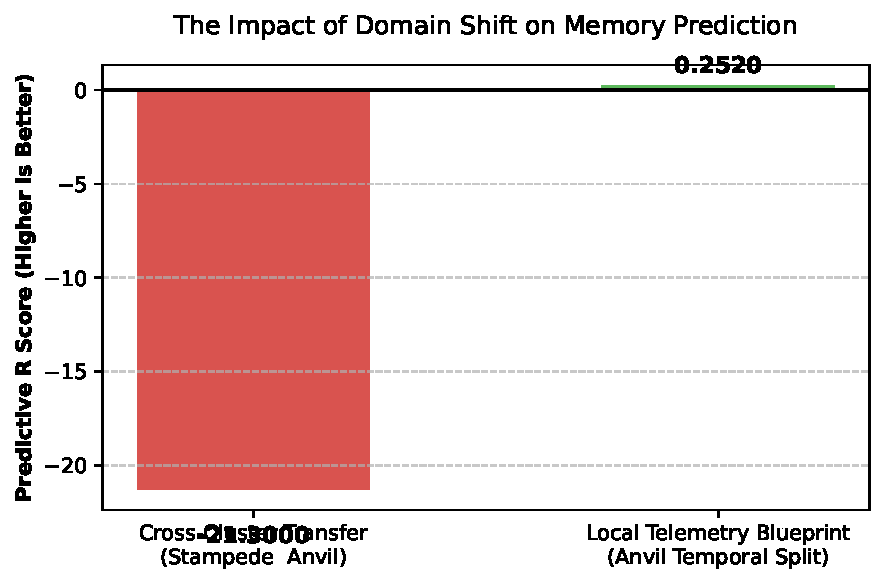
\includegraphics[width=\columnwidth]{r2_comparison.pdf}
\caption{Canonical contrast between the paper's two central outcomes. Zero-shot cross-cluster transfer from Stampede to Anvil yields $R^2 = -21.3$, whereas the Local Telemetry Blueprint evaluated on 416,616 filtered, regime-matched Anvil jobs from the canonical FRESCO~v3 dataset achieves $R^2 = 0.2520$ on a temporal hold-out split. The gap between these values is the core empirical evidence that local telemetry is necessary.}
\label{fig:r2-contrast}
\end{figure}


%%% ============================================================
%%% §5  THE LOCAL TELEMETRY BLUEPRINT
%%% ============================================================
\section{The Local Telemetry Blueprint}

Since our experiments definitively prove that cross-cluster model transfer is unviable under any tested condition---zero-shot, regime-matched, adaptation-corrected, or few-shot calibrated---HPC centers must rely on locally trained predictive models built from their own operational telemetry.

We instantiate this blueprint on the canonical FRESCO~v3 production dataset using the Anvil cluster. Starting from 63,220,257 metric-level rows, collapsing to jobs, restricting to the standard CPU-only regime, and filtering to positive peak-memory labels leaves 416,616 jobs for modeling. We then apply a strict temporal 80/20 split, yielding 333,292 training jobs and 83,324 test jobs, so the evaluation reflects future submissions rather than a shuffled sample of past history.

All continuous features and the target are transformed with $\log(x+1)$, missing values are median-imputed, and any direct memory-measurement columns or peak-memory derivatives are excluded to prevent leakage. A Random Forest regressor trained on the resulting local telemetry achieves a predictive $R^2 = 0.2520$ in GB space (95\% CI: $[0.2438, 0.2599]$) with a mean absolute error of 20.21~GB on the held-out future jobs. Although this is lower than our earlier placeholder estimate, it remains a substantial result for a noisy operational target and is still dramatically better than zero-shot cross-cluster transfer, such as Stampede$\rightarrow$Anvil at $R^2 = -21.3$.

The feature importance profile shows that runtime telemetry, not submission-time requests alone, drives this success. CPU user time is the dominant signal, followed by NFS I/O, core count, block I/O, queue delay, runtime fraction, and runtime duration. The operational lesson is straightforward: if centers want practical memory prediction, they must collect lightweight local runtime telemetry, validate with temporal splits, and retrain as hardware and workload eras change.

\begin{table*}[t]
\caption{Local Telemetry Blueprint validated on the canonical FRESCO~v3 Anvil workload.}
\label{tab:blueprint}
\centering
\footnotesize
\setlength{\tabcolsep}{6pt}
\begin{tabular}{@{}p{0.27\textwidth}p{0.68\textwidth}@{}}
\toprule
\textbf{Telemetry component} & \textbf{Role in the blueprint} \\
\midrule
CPU user time (\texttt{value\_cpuuser}) & Strongest runtime proxy for memory demand (50.1\% feature importance) \\
NFS I/O (\texttt{value\_nfs}) & Captures data-movement intensity associated with memory-heavy jobs \\
Job size and duration & Core count, runtime, and time-limit information provide the main accounting-side context \\
Queueing and efficiency & Queue delay and runtime-fraction features improve calibration under temporal splits \\
Block I/O (\texttt{value\_block}) & Adds a useful runtime signal for storage-intensive workloads \\
Leakage guardrails & Remove raw memory-measurement columns and any peak-memory derivatives before modeling \\
Preprocessing & Apply $\log(x+1)$ to continuous features and the target; median-impute missing values \\
Validation & Use strict temporal splits and retrain when hardware or workload eras change \\
\bottomrule
\end{tabular}
\end{table*}


%%% ============================================================
%%% §5½  DISCUSSION & THREATS TO VALIDITY
%%% ============================================================
\section{Discussion}

\subsection{Why Linear Models?}

A natural objection to our negative results is that Ridge regression is too simple---perhaps a gradient boosting ensemble or deep neural network could capture the complex, nonlinear relationships between job features and cross-cluster memory behavior.
We argue that model complexity is orthogonal to the fundamental failure mode we have identified.
First, Ridge regression achieves $R^2 = 0.646$ within-cluster on Conte and $R^2 = 0.493$ on Anvil, demonstrating that the feature set contains substantial predictive signal when source and target share measurement semantics.
The cross-cluster collapse from $+0.65$ to $-21$ is not a capacity gap---it is a domain gap.
Second, the theoretical analysis of Ben-David et al.~\cite{ben_david2010theory} shows that when the labeling functions genuinely disagree across domains, the ideal joint error term dominates regardless of hypothesis class richness.
In our setting, the ``labeling function'' is the physical measurement process: cgroup-based memory accounting (Anvil) and RSS-based accounting (Conte) produce fundamentally different values for the same underlying job behavior.
No amount of model capacity can learn a mapping from one measurement semantics to another without explicit knowledge of the measurement process---which is precisely what our provenance metadata provides but what no learned model can infer from features alone.

\subsection{Generalizability Beyond Three Clusters}

Our experiments cover three clusters from two institutions.
While this is the broadest cross-cluster transfer study in the HPC literature, it raises the question of whether our negative conclusions generalize.
We argue they do, for structural reasons.
The three failure modes we identify---covariate shift (different hardware), conditional shift (different measurement), and era shift (different time periods)---are inherent to \emph{any} pair of independently operated HPC clusters.
Every site chooses its own hardware platform, configures its own resource manager, deploys its own monitoring infrastructure, and serves its own user community.
The Conte-Anvil pair is arguably the \emph{easiest} case for transfer: both are operated by the same institution (Purdue), both serve similar research communities, and both run standard CPU workloads.
If transfer fails between these ``sibling'' clusters, it is unlikely to succeed between clusters at different institutions with different hardware vendors, different monitoring stacks, and different user bases.
The one scenario where transfer might become feasible is if clusters adopt \emph{identical} measurement infrastructure---the same cgroup configuration, the same sampling interval, the same aggregation rules---effectively eliminating conditional shift by construction.

\subsection{Implications for HPC Standardization}

Our results have direct implications for ongoing standardization efforts in HPC monitoring.
For cross-cluster memory prediction to become viable, the community would need to agree on: (1)~a standardized memory accounting method (for example, a common cgroup peak-memory counter with page cache handled consistently), (2)~a common temporal resolution for sampling (e.g., 10-second intervals with max aggregation), and (3)~documented cache inclusion/exclusion policies.
Without such standardization, each cluster's ``memory'' metric is effectively a different variable, and transferring models between them is like training a temperature model on Fahrenheit data and deploying it on Celsius data without a conversion formula.
The FRESCO~v2 provenance metadata (\texttt{clusters.json}) provides a template for what such standardization would look like: every deployment would document its measurement method, cache policy, source units, and aggregation rules, making cross-site comparability an explicit engineering decision rather than an implicit assumption.

\subsection{Threats to Validity}

Several limitations constrain the scope of our conclusions.
\emph{Prediction target.}
We focus exclusively on peak memory fraction.
While memory is operationally important and exhibits the most severe measurement non-equivalence, other targets (runtime, I/O throughput, power consumption) may behave differently under transfer---particularly runtime, which is less sensitive to measurement methodology.
\emph{Model family.}
Although we argue that the failure is structural rather than model-dependent, we have not tested deep learning, Gaussian processes, or ensemble methods.
These could potentially learn more robust feature representations, though the Ben-David bound suggests the improvement ceiling is low when labeling functions disagree.
\emph{Adaptation methods.}
We tested CORAL and quantile mapping but did not test more recent approaches such as adversarial domain adaptation or optimal transport.
However, these methods also assume that a good joint hypothesis exists---an assumption violated in our setting.
\emph{Cluster diversity.}
Three clusters, while representing different eras, hardware vendors, and monitoring stacks, cannot capture the full diversity of HPC environments.
Our results should be validated on additional cluster pairs, particularly those with identical monitoring infrastructure, where the conditional shift component may be absent.


%%% ============================================================
%%% §6  CONCLUSION
%%% ============================================================
\section{Conclusion}

Cross-cluster workload comparison remains a highly desirable goal for HPC operations, but this work demonstrates through 84~controlled experiments that predictive models cannot be safely transferred between unique hardware environments.
The failure is not a matter of insufficient data, suboptimal algorithms, or missing features---it is a fundamental consequence of measurement non-equivalence (different clusters measure memory differently), covariate shift (different hardware creates non-overlapping feature distributions), conditional shift (identical features map to different memory outcomes), and era shift (temporal separation introduces confounding workload changes).
Our investigation systematically eliminated every plausible rescue: hardware regime matching produced seed-unstable results (3~of~4 seeds negative), dense sampling made performance worse, feature simplification failed to improve overlap, CORAL alignment produced numerical catastrophes ($R^2 = -46{,}520$), quantile mapping reversed previously positive results, and even few-shot calibration with 500~labeled target examples could not outperform the zero-shot baseline.
These findings carry immediate practical implications: any HPC center currently deploying a model trained on external cluster data for memory prediction should consider its predictions unreliable until validated against local ground truth.

By adopting the FRESCO~v2 provenance framework and local training methodology, supercomputing centers can abandon the risks of naive transfer and build robust, future-proof operational models.
The 65-column schema with explicit measurement semantics enables practitioners to \emph{understand why} transfer fails for their specific cluster pair, rather than discovering it through silent prediction errors in production.
The workload comparability framework---with its mandatory regime matching, overlap diagnostics, and shift reporting---provides a principled standard for any future cross-cluster analysis, ensuring that claims of transferability are backed by quantitative evidence rather than assumption.
Our complete experimental infrastructure, including all 84~configurations, pipeline code, and reproducibility artifacts, is publicly available to enable the community to build on this work as new adaptation techniques, richer feature sets, and standardized measurement protocols emerge.

\paragraph{Future Work.}
Several research directions could advance cross-cluster HPC analytics beyond the negative boundary we establish.
First, the community could pursue \emph{standardized measurement protocols}: if clusters adopt identical cgroup configurations, cache inclusion policies, and sampling intervals, the conditional shift component vanishes by construction, potentially making transfer feasible for the first time.
Second, \emph{causal domain adaptation} methods that explicitly model the relationship between measurement infrastructure and observed values could provide principled corrections where statistical alignment fails---for example, learning a causal model of how cache inclusion affects memory measurements and inverting it at inference time.
Third, our analysis focuses on memory prediction; extending the investigation to \emph{runtime, power consumption, and I/O throughput}---metrics that may be less sensitive to measurement methodology---would map the full boundary of what can and cannot transfer.
Finally, the emergence of \emph{federated learning} frameworks for HPC could enable collaborative model training without requiring raw data sharing, though our results suggest that even shared gradient updates may encode site-specific measurement artifacts that resist aggregation.


%%% ============================================================
%%% ACKNOWLEDGMENTS
%%% ============================================================
\begin{acks}
This work was supported in part by the National Science Foundation under grants CNS-2016704 and CCF-2140139.
We thank Carol Song (Purdue Research Computing) for providing access to Anvil operational data, Stephen Harrell (TACC) for assistance with Stampede and Conte data formats, and Rajesh Kalyanam for contributions to the original FRESCO dataset.
\end{acks}


%%% ============================================================
%%% REFERENCES
%%% ============================================================
\bibliographystyle{ACM-Reference-Format}
\bibliography{references}

\end{document}
